\section{Method}
discuss your approach for solving the problems that you set up in the introduction. Why is your approach the right thing to do? Did you consider alternative approaches? It may be helpful to include figures, diagrams, or tables to describe your method or compare it with others.


\begin{table}[!ht]
    \begin{center}
        \caption{Alcune tabelle ordinate per dimensione}
        \label{tab:dim_ordered_tables}
        \rowcolors{2}{gray!25}{white}
        \begin{tabular}{l|l}
            \rowcolor{gray!50}
            \textbf{Nome tabella} & \textbf{Dimensione (MB)} \\
            \hline
            TrendTimeSlotHour & 39667.92\\
            TrendTAInst & 37575.00\\
            TrendTimeSlotSmartInfo & 25276.00\\
            TrendTAHour & 19270.95\\
            TrendWMeterInst & 16196.00\\
            TrendTAEnergyHour & 11697.28\\
            TrendPlant & 8537.20\\
            TrendRefHour & 4989.47\\
            TrendWMeterHour & 4896.97\\
            ... & ...\\
            \hline
        \end{tabular}
    \end{center}
\end{table}
\cite{ms_excel}

\paragraph{Estrazione dei dati mancanti}
data la mancanza dell'energia prodotta, consumata e quindi venduta e acquistata, si è dovuto provvedere al suo calcolo. L'energia è calcolabile attraverso la potenza \(P\) e l'intervallo di tempo \(\delta T\) secondo la formula: 
\(E = P\times \delta T \)
La potenza invece, essendo i sistemi mono, bi e trifase e attiva e reattiva, è stata calcolata con:
$\ P = \sqrt{\sum_{f=1}^{3} P_f^{2} + \sum_{f=1}^{3} Q_f^{2}}$
dette \(P_f\) e \(Q_f\) rispettivamente la potenza attiva e reattiva.

\begin{figure}[!ht]
    \centering
    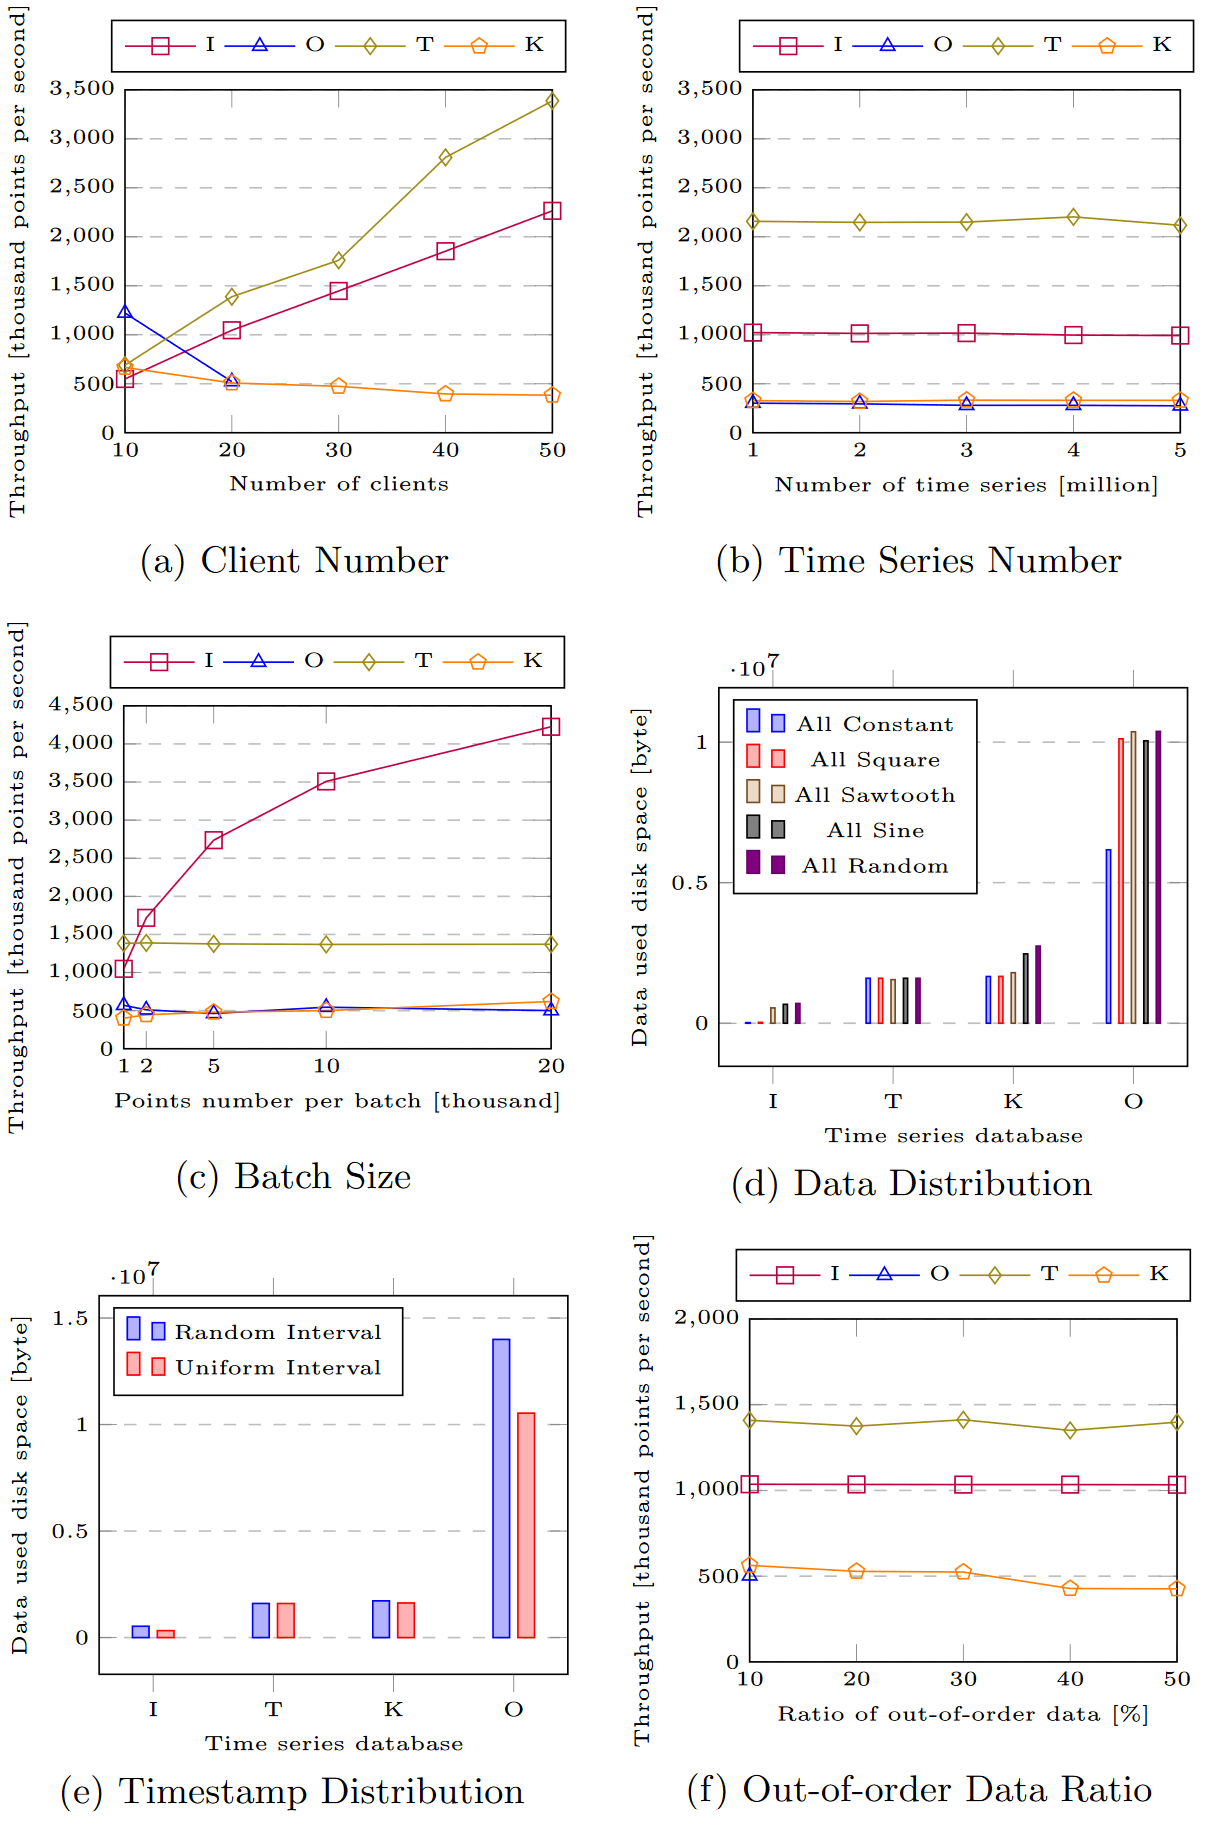
\includegraphics[scale=0.34]{images/data_ingestion_benchmark.png}
    \caption{Esperimenti di ingestione di dati. I, T, K e O individuano InfluxDB, TimescaleDB, KairosDB e OpenTSDB.}
    \label{tab:data_ingestion_benchmark}
\end{figure}

%%%%%%%%%%%%%%%%%%%%%%%%%%%%%%%%%%%%%%%%%%%%%%%%%%%%%%%%%%%%%%%%%%%%%%%%%%%%%%%%%%%%%%%%%%%%%%%%%%%%

